% this figure is contained here because it messes up
% syntax highlighting for the rest of whatever file
% it's in. the reason is that the highlighter doesn't
% understand that we're switching between tex, python
% and regexes.

\begin{figure}[htb]
\centering
\begin{minted}[linenos,breaklines,frame=single,xleftmargin=1cm,breakindent=0em,breaksymbolindentleft=0em]{python}
# salutations and exclamations that cause parser errors
badwords = ['-l.b-', 'hi', 'hey', 'hello', 'oh', 'wow',
            'thankyou', 'thanks', 'welcome',  'thank']

# mood types as dict object
m = {'Mod. declarative':
       r'ROOT < (S < (/(NP|SBAR|VP)/ $+ (VP < MD)))',
     'Unmod. declarative':
       r'ROOT < (S < (/(NP|SBAR|VP)/ $+ (VP !< MD)))',
     'Interrogative':
       r'ROOT << (/\?/ !< __)',
     'Imperative':
       r'ROOT < (/(S|SBAR)/ < (VP !< VBD !< VBG !$ NP !$ SBAR < NP !$-- S !$-- VP !$ VP)) !<< (/\?/ !< __) !<<- /-R.B-/ !<<, /%s/' % as_regex(badwords)}
\end{minted}
\caption{Tregex queries for Major clause Mood Types}
\label{fig:mood_dict}
\end{figure}

\begin{figure}[htb]
\centering
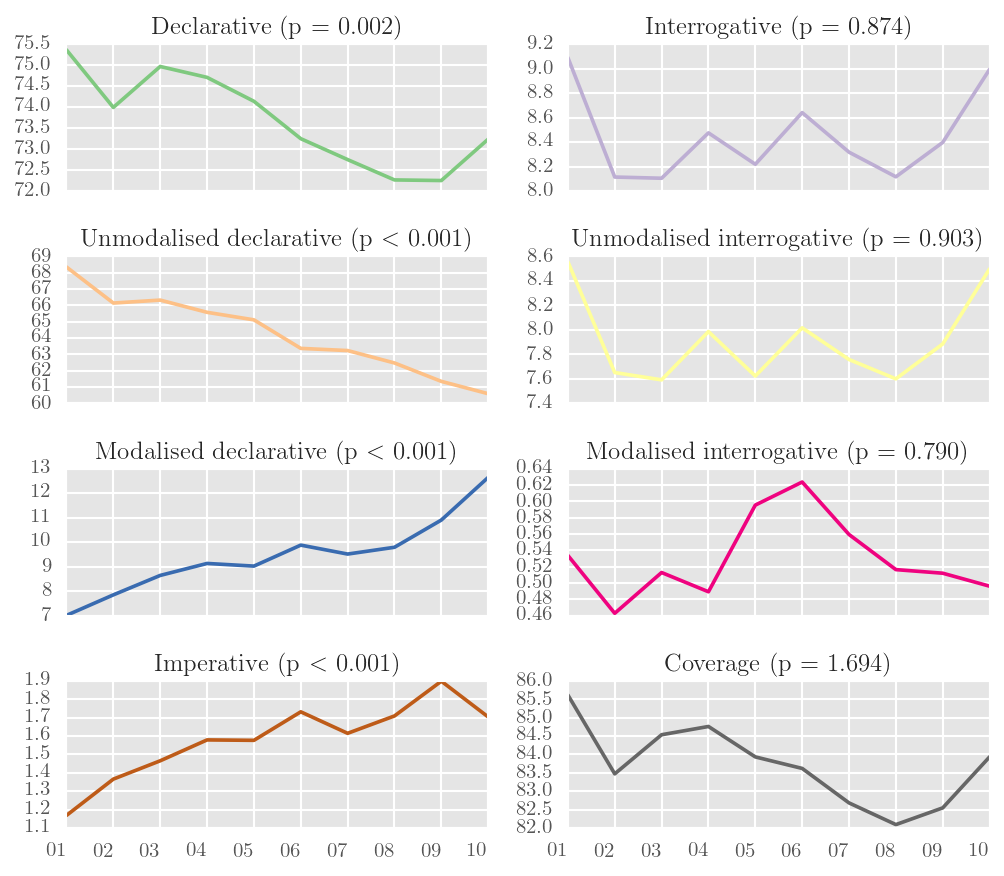
\includegraphics[width=0.8\textwidth]{../images/known-mood-and-indicative-types-in-p-corpus.png}
\caption{Mood features in the Membership Stage Structure}
\label{fig:mood_types_P}
\end{figure}